\scanpage{34}
\uline{Sous-groupes finis de} $\mathrm{GP}(1,k),\mathrm{Sl}(2,k),\mathrm{Gl}(2,k)$

On suppose d'abord $k$ corps de car. 0, alg clos.

a) \uline{Sous groupes finis de} $\mathrm{GP}(1,k)=G$

\uline{Thme} a) Pour que deux ss-groupes finis \inserted{$\Gamma,\Gamma'$} de $G$ soient conjugués
dans $G$, il f. et s. qu'ils soient isomorphes.

b) Les classes d'isom. de sous-groupes finis de $G$
sont \inserted{celles de} $\mathbb Z/n\mathbb Z$ ($n\deleted{\unsure{\geq1}}\deleted{\unsure{\geq2}}$), $\mathbb D_n$ ($n\geq2$), $\mathcal A_4,\unsure{\mathfrak S_4|\mathscr S_4},\mathcal A_5$, i.e.
ce sont \uline{exactmt} les types des groupes d'isom. des
\inserted{cartes orientées régulières sphériques (avec leurs \uline{plongements} naturels ds $\mathrm{GP}(1)$\unsure{.…})}

% slanted

\deleted{c) Si $\Gamma$ est un sous-gpe de $G$, son normalisateur}
\deleted{il est égal à son normalisateur, sauf dans les
cas de $\mathbb Z/n\mathbb Z$ ($n\geq1$) et de $\mathbb D_2$, \inserted{de $\mathcal A_4$.} Dans ces cas
on a, notant à part le cas trivial de $1=\mathbb Z/n\mathbb Z$ \unsure{on a :|inclus :}}
\deleted{on a}

\deleted{1°) \deleted{Normalisateur de} $N(\mathbb Z/n\mathbb Z)$ \deleted{est} \deleted{le normali}\inserted{$N(T)$}, $T=Z(\mathbb Z/n\mathbb Z)$
est l'unique tore maximal qui cont.
$\mathbb Z/n\mathbb Z$, \deleted{Centr.} $N(\mathbb Z/n\mathbb Z)/Z(\mathbb Z/n\mathbb Z)=\mathbb Z/2\mathbb Z$}

\deleted{2°) \deleted{Normalisateur de} $N(\mathbb D_2)\unsure{\Rightarrow|=|\xrightarrow{\sim}}\mathfrak S_4$,}

\[
\begin{aligned}
&\deleted{\text{Centralisateur de}}\quad\deleted{Z(\mathbb D_{\unsure{2|n}})=\mathbb D_2}\\ 
&\deleted{N(\mathbb D_2)/Z(\mathbb D_2)\xrightarrow{\sim}\mathrm{Aut}(\mathbb D_2)\simeq\mathfrak S_3}
\end{aligned}
\]

\[
\begin{aligned}
&\deleted{3^\circ)\quad N(\mathcal A_4)=\mathfrak S_4}\\ 
&\deleted{Z(\mathcal A_4)=(1)}\qquad\deleted{N(\mathcal A_4)/Z(\mathcal A_4)=\mathfrak S_4}\\ 
&\hspace{14em}\deleted{=\mathrm{Aut}(\mathcal A_4)}
\end{aligned}
\]

\figure{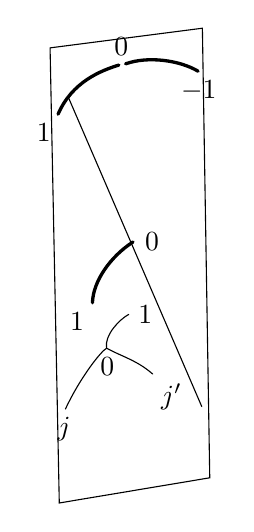
\begin{tikzpicture}[x=.78cm,y=.78cm,line cap=round]
\draw (-.48,6.38)--(2,6.7)--(2.12,-.62)--(-.33,-1.03)--cycle;
\draw[very thick] (-.35,5.3) .. controls (-.12,5.83) and (.35,6.01) .. (.64,6.1);
\draw[very thick] (.75,6.12) .. controls (1.11,6.25) and (1.63,6.18) .. (1.93,6.0);
\node[below left] at (-.31,5.30) {$1$}; \node[above] at (.68,6.09) {$0$}; \node[below] at (1.94,6.0) {$-1$};
\draw[very thick] (.21,2.23) .. controls (.22,2.58) and (.50,2.98) .. (.87,3.22);
\node[below left] at (.23,2.23) {$1$}; \node[right] at (.91,3.22) {$0$};
\draw (-.23,.5) .. controls (.02,1.03) and (.35,1.44) .. (.44,1.49) .. controls (.70,1.35) and (.94,1.29) .. (1.19,1.07);
\draw (.44,1.49) .. controls (.4,1.70) and (.65,1.96) .. (.80,2.04);
\node[below] at (.45,1.50) {$0$}; \node[right] at (.8,2.04) {$1$}; \node[below] at (-.25,.53) {$j$}; \node[below right] at (1.17,1.07) {$j'$};
\draw[thin] (-.18,5.57)--(1.99,.54);
\end{tikzpicture}}

\deleted{D'autre part, dans tous les cas sauf}

\deleted{c) Pour toute carte \deleted{\unsure{$G$}} orientée finie
sphérique (connexe) $\mathcal C$, considérons sa
réalisation topologique -- on trouve un
foncteur de groupoïdes}

\diagram{\begin{tikzcd}[ampersand replacement=\&,column sep=small]
\deleted{\mathcal C}\arrow[r,"{\deleted{\unsure{\sim}}}"]\&\deleted{\substack{\mathcal C=\text{cat. des}\\ \text{``cartes holomorphes sphériques'',}\\ \text{i.e. des ``cartes h.\unsure{lomorphes}''}\\ \deleted{\text{sur}}\ \text{telles que la variété}\\ \text{complexe sous-jacente}\\ \text{soit }\deleted{\text{de}}\ \unsure{\text{simple}|\text{sphère}|\text{de type}}\ \text{de genre 0}}}\arrow[r]\&\deleted{\substack{\text{catégorie}\\ \text{des couples}\\(G,\Gamma)\ \text{d'une}\\\text{forme de}\\\mathrm{GP}(1,\mathbb C)\\\text{et d'un}\\\text{sous-gp.}\\\text{fini }\Gamma}}
\end{tikzcd}}

% archive sheet number: 33
